\documentclass[11pt, a4paper]{article}

% --- BLOQUE UNIVERSAL DE PREÁMBULO ---
\usepackage[a4paper, top=2.5cm, bottom=2.5cm, left=2.5cm, right=2.5cm]{geometry}
\usepackage{fontspec}
\usepackage[main=spanish, english]{babel}

% Configuraciones de Babel y Fuentes
% Usamos Noto Sans para un look moderno y limpio (Mandatorio)
\babelfont{rm}{Noto Sans}

% Paquetes adicionales para estética y funcionalidad
\usepackage{xcolor}
\usepackage{titlesec}
\usepackage{enumitem}
\usepackage[most]{tcolorbox}
\usepackage{amsmath}
\usepackage{amsfonts}
\usepackage{booktabs}
\usepackage{pagecolor}
\usepackage{caption}
\usepackage{array}
\usepackage{ragged2e}
\usepackage{setspace}
\usepackage{xcolor}
\usepackage{enumitem}
\usepackage{float}

% --- DEFINICIÓN DE COLORES ---
\definecolor{fondo}{HTML}{E5CCAB} % Color crema solicitado
\definecolor{primario}{HTML}{2D3E50} % Azul oscuro para texto
\definecolor{acento}{HTML}{8C4646}   % Bordó para títulos y énfasis
\definecolor{cajaCuerpo}{HTML}{F5E6D3} % Color suave para fondo de cajas

% Aplicar color de fondo a la página
\pagecolor{fondo}
\color{primario}

% --- ESTILO DE SECCIONES ---
\titleformat{\section}
{\color{acento}\normalfont\Large\bfseries}
{\thesection}{1em}{}[{\titlerule[0.8pt]}]

\titleformat{\subsection}
{\color{acento}\normalfont\large\bfseries}
{\thesubsection}{0.8em}{}[{\color{acento!80}\titlerule[0.5pt]}]

\titleformat{\subsubsection}
{\color{acento!90}\normalfont\normalsize\bfseries}
{\thesubsubsection}{0.7em}{}

\titlespacing*{\section}{0pt}{1.3em}{0.8em}
\titlespacing*{\subsection}{0pt}{1.1em}{0.6em}
\titlespacing*{\subsubsection}{0pt}{0.9em}{0.4em}

\setstretch{1.4}

% --- CONFIGURACIÓN DE CAJAS (tcolorbox) ---
% Se corrige el error de "sharp corners=false" eliminando la opción conflictiva
\newtcolorbox{definicion}[1]{
  colback=cajaCuerpo,
  colframe=acento,
  fonttitle=\bfseries,
  title=#1,
  arc=3mm,
  boxrule=0.6mm,
  left=4mm,
  right=4mm,
  top=3mm,
  bottom=3mm
}

\newtcolorbox{nota}{
  colback=white!40!fondo,
  colframe=primario!60,
  arc=2mm,
  boxrule=0pt,
  leftrule=2mm,
  fontupper=\small\itshape,
  breakable
}

\setlist[enumerate]{leftmargin=4em}
\setlist[itemize]{leftmargin=4em}
\captionsetup[figure]{font=it, labelfont=it}


% --- DATOS DEL DOCUMENTO ---
\title{
    \vspace{-1.5cm}
    \textbf{\huge Redes de Datos II}\\
    \vspace{0.5cm}
    \large Facultad de Informática --- UNLP
}
\author{\textit{Taciano Pacchialat}}
\date{\the\year}

% Hipervínculos (siempre al final del preámbulo)
\usepackage[colorlinks=true, linkcolor=acento, urlcolor=acento]{hyperref}

\begin{document}

\maketitle

\begin{abstract}
    \noindent Este documento es una guía estructurada para el repaso de los contenidos fundamentales de la materia. Se enfoca en la claridad visual y la jerarquización de conceptos mediante el uso de colores y bloques resaltados.
\end{abstract}

\tableofcontents
\newpage

\section{Address Resolution Protocol (ARP)}

ARP es un protocolo de capa 2 (capa de enlace), que trabaja con Ethernet y otros protocolos de capa 2 para ayudar a IP. Es un protocolo \textbf{helper} de IP. Su función principal es mapear direcciones lógicas a físicas (mapear dirección IP a dirección MAC). Utiliza auto-aprendizaje, no requiere de configuración (es dinámico). Es encapsulado dentro de una trama Ethernet.

\begin{nota}{\textbf{Recordar} \newline}
    ARP funciona dentro de un dominio de \emph{broadcast}, no permite determinar la dirección MAC de un dispositivo en otra red.
\end{nota}

Cada nodo tiene una tabla ARP en memoria que contiene la relación entre una IP y una MAC. 

\subsection{Funcionamiento de ARP}

Supongamos que PC-A y PC-B están en un mismo dominio de broadcast. Si A le quiere enviar un mensaje a B, debe primero conocer su dirección MAC. Por la IP A sabe que B está en su misma red, entonces envía un \textbf{ARP Request} a la MAC de broadcast (ff:ff:...:ff) con la IP a la que debe enviarle el mensaje.

\begin{figure}[htbp]
    \centering
    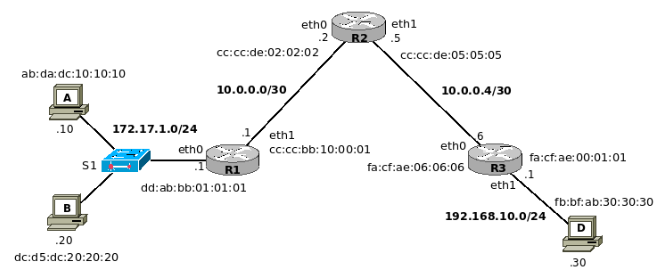
\includegraphics[width=0.7\textwidth]{capitulos/arp/imagenes/topologia-ejemplo.png}
    \caption{Topología del ejemplo}
    \label{fig:ejemplo-arp}
\end{figure}

El nodo que tenga la IP destino asignada, procesará y responderá al ARP Request con un \textbf{ARP Reply} de tipo unicast. Una vez respondido, A ya puede enviarle mensajes a B por tener su dirección física. 

Ahora supongamos que PC-A le quiere enviar un mensaje a PC-D, que está en \textbf{otra red}. Para llegar a D, A debe encontrar la MAC de su \emph{default gateway}. El procedimiento es el mismo que para el caso anterior: ARP Request a la dirección de broadcast y el router de gateway responde con un ARP Reply.

Ahora, A envía el mensaje \textbf{Echo Request} con la interfaz del router como MAC destino. Cuando llega el mensaje, el router rutea el paquete y lo pasa a la capa inferior para forwardearlo por la interface que corresponda. El paquete puede ser enviado a otro router o al destino final, y si el router no conoce la MAC destino debe volver a ejecutar ARP para cambiar los campos de la trama Ethernet. 

\newpage

\section{Protocolo IP}

La \textbf{capa de enlace} (capa 2) se encarga de proveer conectividad entre nodos adyacentes o vecinos, siendo responsable de transmitir una trama sobre un enlace en particular. Los mensajes entre origen y destino pueden transitar por distintas capas de enlace. La \textbf{Capa de Red} se encuentra por encima de la capa de enlace.

\begin{figure}[htbp]
    \centering
    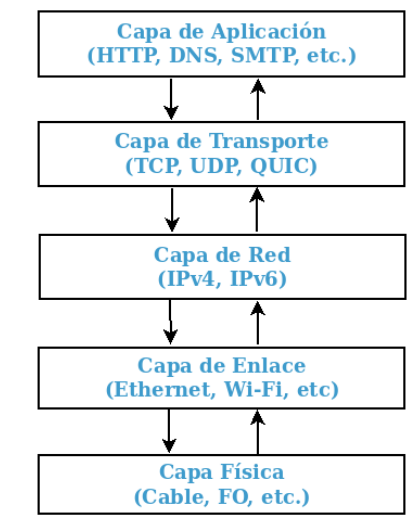
\includegraphics[width=0.5\textwidth]{capitulos/ip/imagenes/capas.png}
    \caption{Modelo TCP/IP}
    \label{fig:capas-de-modelo-tcp}
\end{figure}

\subsection{Diseño y Servicios}

La capa de red fué diseñada para que cumpla con los siguientes requerimientos: 

\noindent
\begin{enumerate}[label=\textcolor{acento}{$\bullet$}]
    \item Independiente de la tecnología de subred.
    \item Aislada de la cantidad, tipo y topologías de las \textbf{subredes}.
    \item Direccionamiento uniforme.
\end{enumerate}

Como servicios, debe poder transportar mensajes desde un nodo emisor a receptor (inclusive si son redes distintas) y determinar el camino que seguirá un mensaje entre dos nodos. Al no ser orientado a conexión, no brinda ni control de errores, ni secuenciamiento ni confiabilidad: es un servicio de \textbf{Best-Effort}.

\begin{definicion}{Protocolo Best-Effort}
    Hay independencia en cuanto al envío a través de la red, haciendo posible que los paquetes puedan llegar desordenados o seguir caminos diferentes. Tampoco hay control de errores. 
\end{definicion}

Tiene dos funcionalidades principales:

\begin{itemize}[label=\textcolor{acento}{$\bullet$}]
    \item Direccionamiento
    \item Ruteo
\end{itemize}

También se encarga de multiplexar o demultiplexar protocolos superiores, y puede fragmentar paquetes.

\begin{figure}[htbp]
    \centering
    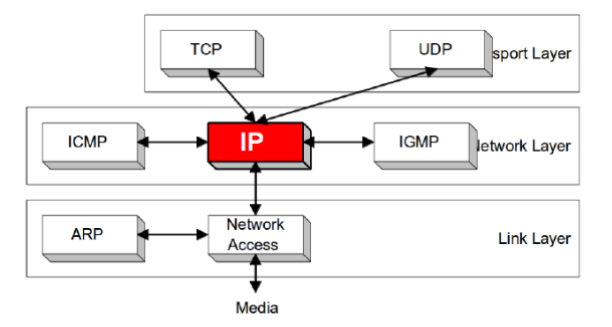
\includegraphics[width=0.5\textwidth]{capitulos/ip/imagenes/capas-relativo-ip.png}
    \caption{Modelo TCP/IP}
    \label{fig:capas-relativo-ip}
\end{figure}

\subsection{Estructura del Datagrama IP}

El \textbf{Datagrama IP} tiene longitud variable. Está compuesto por dos partes: header y payload. El \textbf{Header} tiene una longitud de entre 20 y 60 bytes.

\begin{figure}[htbp]
    \centering
    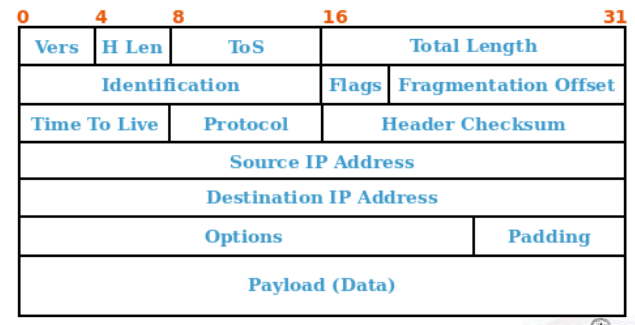
\includegraphics[width=0.5\textwidth]{capitulos/ip/imagenes/ip-datagram.png}
    \caption{Datagrama IP}
    \label{fig:ip-datagram}
\end{figure}

Los campos más relevantes son: 

\begin{itemize}[label=\textcolor{acento}{$\bullet$}]
    \item \textbf{Header Lenght:} longitud del header, en palabras de 32 bits.
    \item \textbf{Type of Service (TOS):} confiabilidad, prioridad, retardo y throughput.
    \item \textbf{Identification:} número único para segmentos del mismo datagrama.
    \item \textbf{Flags:} 
    \begin{itemize}[label=\textcolor{primario!60}{$\bullet$}]
        \item X = reservado. 
        \item D = Don't Fragment. Si es 0 puede fragmentarse, si es 1 no.
        \item M = More Fragments. Si es 0 es el último fragmento, si es 1 no.
    \end{itemize}
    \item \textbf{Fragment Offfset:} el desplazamiento del segmento dentro del datagrama original. Está dado en múltiplos de 8 bytes.
    \item \textbf{Time To Live (TTL):} número que se decrementa cada vez que llega a un router, y cuando llega a 0 se descarta. Es utilizado para evitar loops.
    \item \textbf{Protocol:} protocolo contenido en el campo de datos (UDP, TCP, ICMP, ...).
\end{itemize}

\subsection{Direccionamiento IP}

Las direcciones IP identifican unívocamente una intefraz de red. Los routers pueden tener más de una dirección IP, y a diferencia de las direcciones MAC, estas direcciones son lógicas.

Hay distintos tipos de direcciones: 

\begin{itemize}[label=\textcolor{acento}{$\bullet$}]
    \item \textbf{Unicast:} destinada a un host/interface en particular.
    \item \textbf{Broadcast:} destinada a todos los hosts de una red.
    \item \textbf{Multicast:} destinada a un grupo de hosts de una o varias redes.
\end{itemize}

Además de estas direcciones, también está la de \emph{Loopback} (127.0.0.1) y la utilizada cuando aún no se le asignó una red al dispositivo (0.0.0.0).

\subsubsection{Subnetting}

El subnetting es el proceso de dividir una red física o lógica de gran tamaño en subredes más pequeñas. Esto se logra alterando la máscara de red predeterminada, ``pidiendo prestados'' bits de la porción destinada a los hosts para asignarlos a la porción de red.


\begin{itemize}[label=\textcolor{acento}{$\bullet$}]
    \item \textbf{Objetivo:} Reducir el tamaño de los dominios de broadcast, mejorar la seguridad, facilitar la administración y evitar el desperdicio de direcciones IP dentro de una organización.
    \item \textbf{Mecanismo:} Se desplaza el límite de la máscara de red hacia la derecha (aumenta el prefijo).
    \item \textbf{Cálculo de Subredes y Hosts:} 
    Si se toman $n$ bits prestados de la porción de host, se pueden crear $2^n$ subredes. En cada subred, si quedan $h$ bits para los hosts, habrá $2^h - 2$ direcciones utilizables (se restan 2 por las direcciones de red y de broadcast).
\end{itemize}

\subsection{VLSM (Variable Length Subnet Mask)}
El subnetting tradicional (FLSM) divide una red en subredes del mismo tamaño, lo que a menudo sigue generando desperdicio. \textbf{VLSM} mejora esto permitiendo aplicar diferentes máscaras de subred dentro del mismo bloque de direcciones mayor. Al hacer subnetting de una subred previamente dividida, los bloques se ajustan estrictamente a la cantidad de hosts necesarios para cada departamento o enlace.

\begin{nota}{\textbf{Ejemplo de Subnetting} \newline}
    Dada la red $192.168.10.0/24$, si necesitamos una red para 80 hosts (requiere 7 bits, $2^7-2 = 126$), utilizamos un prefijo $/25$. La dirección sería $192.168.10.0/25$. El segmento sobrante, $192.168.10.128/25$, se puede seguir dividiendo con prefijos mayores (como $/26$, $/27$) para áreas que requieran menos hosts.    
\end{nota}

\subsubsection{Supernetting (Sumarización)}

El supernetting o \textbf{CIDR (Classless Inter-Domain Routing)}, es el proceso conceptualmente opuesto al subnetting. Consiste en combinar o agrupar múltiples redes contiguas más pequeñas en una única red o ruta más grande.

\begin{itemize}[label=\textcolor{acento}{$\bullet$}]
    \item \textbf{Objetivo:} Reducir drásticamente el tamaño de las tablas de ruteo en los routers de núcleo (core routers) de Internet y optimizar el procesamiento de rutas.
    \item \textbf{Mecanismo:} Se desplaza el límite de la máscara de red hacia la izquierda (disminuye el tamaño del prefijo), agrupando los bits de red compartidos.
    \item \textbf{Requisitos para la Sumarización:} Para agrupar redes, estas deben ser contiguas, el número de redes a agrupar debe ser potencia de 2, y las redes deben compartir exactamente los mismos bits de red de orden superior.
\end{itemize}


Ahora un \textbf{ejemplo}. Supongamos que un router tiene en su tabla las siguientes cuatro rutas hacia subredes contiguas:
\begin{itemize}
    \item $192.168.0.0/24$ (En binario el tercer octeto es: $00000000$)
    \item $192.168.1.0/24$ (En binario el tercer octeto es: $00000001$)
    \item $192.168.2.0/24$ (En binario el tercer octeto es: $00000010$)
    \item $192.168.3.0/24$ (En binario el tercer octeto es: $00000011$)
\end{itemize}

Dado que las cuatro redes comparten los primeros 22 bits ($192.168.000000XX$), se pueden agrupar en una única entrada en la tabla de enrutamiento reduciendo la máscara a $/22$. La ruta resumida resultante será:
$$\mathbf{192.168.0.0/22}$$

\subsubsection{Cuadro Comparativo}
\small
\setlength{\tabcolsep}{4pt}
{\renewcommand{\arraystretch}{1.5}
\begin{table}[h!]
\centering
\begin{tabular}{@{} >{\RaggedRight\arraybackslash}p{3.8cm} >{\RaggedRight\arraybackslash}p{5.3cm} >{\RaggedRight\arraybackslash}p{5.3cm} @{}}
\toprule
\textbf{Característica} & \textbf{Subnetting} & \textbf{Supernetting (CIDR)} \\
\midrule
\textbf{Definición} & Divide una red en redes más pequeñas. & Agrupa redes pequeñas en una más grande. \\
\textbf{Movimiento de Máscara} & Hacia la derecha (aumenta el prefijo, ej. $/24 \rightarrow /26$). & Hacia la izquierda (reduce el prefijo, ej. $/24 \rightarrow /22$). \\
\textbf{Problema que Resuelve} & Agotamiento interno de IPs y dominios de broadcast grandes. & Crecimiento desmedido de las tablas de ruteo globales. \\
\textbf{Bits alterados} & Toma bits de \textit{Host} para hacer \textit{Red}. & Toma bits de \textit{Red} para hacer \textit{Host}. \\
\bottomrule
\end{tabular}
\end{table}
}

\subsection{Routing}

Acción donde se selecciona el próximo salto de un paquete, y su interfaz de salida. Los routers y hosts pueden hacer routing. Es una acción de control, cuyo motor son los protocolos de enrutamiento. Las tablas de ruteo estan compuestas por:

\begin{itemize}[label=\textcolor{acento}{$\bullet$}]
    \item Red Destino
    \item Máscara de Red (o Prefijo)
    \item Next Hop (Próximo Salto)
    \item Interface de Salida
    \item Métrica
\end{itemize}

\begin{nota}{\textbf{Recordar} \newline}
    Solo puede haber un default gateway por tabla de ruteo.
\end{nota}

A diferencia del routing, el \textbf{Forwarding} consiste en pasar un mensaje desde una interfaz de entrada hacia una de salida, por donde envía los mensajes de los protocolos enrutados. 

\subsection{Fragmentación}

\begin{definicion}{Maximum Transfer Unit (MTU)}
    Es el tamaño máximo de paquete permitido en un enlace. 
\end{definicion}

Un datagrama puede pasar por varias capas de enlaces con distintos MTUs, y los datagramas con tamaño mayor al MTU deben ser fragmentados con tamaño \textbf{múltiplo de 8 bytes} (excepto el último). Cada fragmento pasa a ser un nuevo paquete, donde el header se copia del original y luego se modifican los campos necesarios. 

El \textbf{Path MTU} permite saber el mínimo MTU entre origen y destino.


\begin{figure}[htbp]
    \centering
    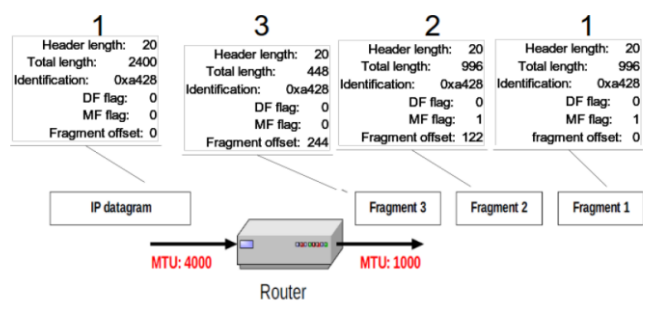
\includegraphics[width=0.5\textwidth]{capitulos/ip/imagenes/fragmentacion.png}
    \caption{Fragmentación en IP}
    \label{fig:fragmentacion-ip}
\end{figure}

Los datagramas se reconstruyen en el destino final una vez que llegan todos los fragmentos, que pueden tomar distintos caminos. Estos fragmentos pueden a su vez fragmentarse de nuevo. En caso de que no lleguen \textbf{todos} los fragmentos, el paquete entero se descarta.









\newpage

\section{Internet Control Message Protocol (ICMP)}

Protocolo helper de IP completamente \textbf{informativo}, es decir, no toma decisiones sino que permite reportar errores o consultar información. Tampoco agrega confiabilidad, sino que \textbf{brinda feedback}. Se encapsula en IP, pero no es un protocolo de transporte.


Cuando un dispositivo descarta un datagrama IP, genera un mensaje ICMP que incluye el encabezado (header) del datagrama original que produjo el problema y al menos los primeros 8 bytes del campo de datos de dicho datagrama.

Los mensajes ICMP son los siguientes.

\subsection{Mensajes de Error (Error-reporting messages)}
Estos mensajes reportan errores que un dispositivo puede encontrar cuando procesa un paquete IP.

\begin{itemize}[label=\textcolor{acento}{$\bullet$}]
    \item \textbf{Destination Unreachable (Tipo 3):} Indica que el paquete no pudo llegar a su destino.
    \begin{itemize}[label=\textcolor{acento!60}{$\bullet$}]
        \item \textit{Code 0:} Net Unreachable (Red inalcanzable).
        \item \textit{Code 1:} Host Unreachable (Host inalcanzable).
        \item \textit{Code 3:} Port Unreachable (Puerto inalcanzable, muy común al fallar una conexión UDP).
    \end{itemize}
    
    \item \textbf{Time Exceeded (Tipo 11):} Se genera cuando expira un temporizador relacionado al datagrama.
    \begin{itemize}[label=\textcolor{acento!60}{$\bullet$}]
        \item \textit{Code 0:} In Transit. Se venció el campo TTL (Time to Live) durante el tránsito por los routers.
        \item \textit{Code 1:} Reassembly Timeout. Se descartó un datagrama fragmentado porque se agotó el tiempo de espera antes de que llegaran todos sus fragmentos para el reensamblado.
    \end{itemize}
\end{itemize}

\subsection{Mensajes de Consulta (Query messages)}
Estos mensajes ocurren usualmente de a pares (una solicitud y su correspondiente respuesta) y permiten obtener información específica del estado de un dispositivo en la red.

\begin{itemize}[label=\textcolor{acento}{$\bullet$}]
    \item \textbf{Echo Request / Echo Reply (Tipos 8 y 0):} Son los mensajes utilizados por la clásica utilidad de diagnóstico \texttt{ping} para comprobar la conectividad bidireccional entre nodos.
    \item \textbf{Timestamp Request / Timestamp Reply (Tipos 13 y 14):} Utilizados para determinar el tiempo de tránsito a través de la red o para sincronizar relojes de los dispositivos.
\end{itemize}


Cuando un mensaje ICMP es descartado, \textbf{no se genera otro} para avisar que se descartó (evito bucles). Solo avisamos el descarte de un fragmento si es el \textbf{primero}, y tampoco avisamos si se descarta un mensaje con destino multicast.

\newpage

\section{Dynamic Host Configuration Protocol - DHCP}

Permite una asignación automática de dirección al nodo, con parámetros de configuración que recibe desde un servidor. Se ejecuta \textbf{encapsulado en UDP}; los clientes escuchan en el puerto 68 y los servidores en el 67.

DHCP contiene dos componentes: un protocolo para enviar parámetros de configuración desde el servidor DHCP a los hosts, y otro para alocar las direcciones de red a los hosts. Los mecanismos para alocar una dirección IP son tres: 

\begin{itemize}[label=\textcolor{acento}{$\bullet$}]
    \item \textbf{Automatic Allocation:} asigna una dirección a un cliente permanentemente.
    \item \textbf{Dynamic Allocation:} asigna una dirección por tiempo limitado.
    \item \textbf{Manual Allocation:} la dirección se asigna por el administrador de red y DHCP solo se la transporta al cliente.
\end{itemize}

Este protocolo utiliza un \textbf{pool de direcciones}, que representa el rango de direcciones que el servidor puede asignar. Cuando se asigna una dirección se hace con un \textbf{lease}, que representa el tiempo por el que un host puede utilizar esa dirección. El host puede pedir una renovación del lease con otra solicitud. 

Cuando el cliente solicita una IP también pide la máscara de red, el default gateway y un servidor DNS. También puede pedir servidores SMTP, POP, HTTP o NTP.

\subsection{Funcionamiento de DHCP}

DHCP funciona con un procedimiento llamado \textbf{DORA:} Discover, Offer, Request, Acknowledge.

\begin{enumerate}[label=\textcolor{acento}{\textbf{\arabic*.}}]
    \item El cliente envía un broadcast \textbf{DHCP Discovery} usando como origen la \texttt{IP 0.0.0.0}, indicando que no puede recibir unicasts (no tiene dirección).
    \item El servidor (o servidores) responde con un \textbf{DHCP Offer} con una IP de su \emph{pool}.
    \item Si el cliente acepta esa IP, responde con un broadcast \textbf{DHCP Request}. Es broadcast para que los otros servidores sepan que su \emph{Offer} fué rechazado.
    \item El cliente comprueba que esa dirección ofrecida no esté en uso mediante ARP.
    \item El servidor envía u \textbf{DHCP Ack} con parámetros de configuración y termina el proceso
\end{enumerate}

Cuando tenemos varias redes, se suele usar un único servidor DHCP centralizado. Para que esto funcione existen los \textbf{DHCP Relays}, routers que reciben los mensajes broadcast de los clientes y se los reenvían al DHCP Server como unicast. También realiza el proceso inverso. 

\begin{figure}[H]
    \centering
    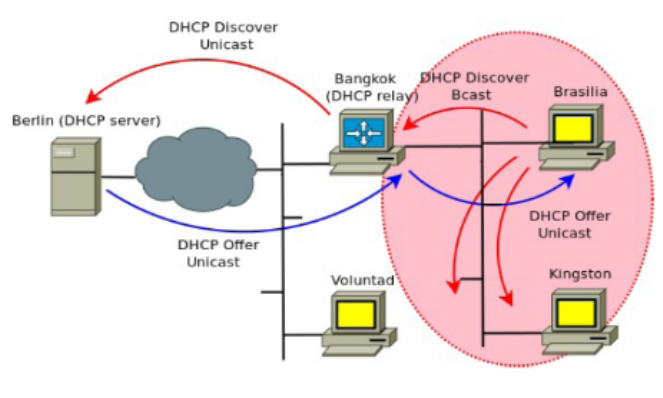
\includegraphics[width=0.5\textwidth]{capitulos/dhcp/imagenes/dhcp-relay.png}
    \caption{Ejemplo de DHCP Relay}
    \label{fig:dhcp-relay}
\end{figure}


\newpage

\section{Protocolo IPv6}

A medida que avanzaba el tiempo, las direcciones IPv4 escaseaban, habían tablas de ruteo muy grandes y mucha congestión entre los routers por exceso de procesamiento. Por esto se introduce un protocolo nuevo: IPv6.


\subsection{Cambios con respecto a IPv4}

Los aspectos modificados son los siguientes:

\begin{itemize}[label=\textcolor{acento}{$\bullet$}]
    \item Direcciones de 128 bits.
    \item No hay más fragmentación.
    \item No hay más header checksum.
    \item El header es de tamaño fijo, sin campo de opciones.
    \item Se extiende el protocolo con cabeceras de extensión.
\end{itemize}

\begin{figure}[htbp]
    \centering
    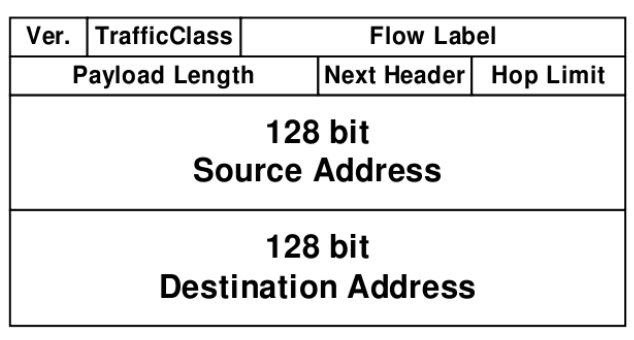
\includegraphics[width=0.5\textwidth]{capitulos/ipv6/imagenes/header-ipv6.png}
    \caption{Header de IPv6}
    \label{fig:header-ipv6}
\end{figure}


\subsection{Direcciones IPv6}

También se modifican los tipos de direcciones: ya no hay direcciones de broadcast, sino que hay unicast, anycast y multicast, que tienen formato \texttt{FF00::/8}.

La notación cambia. Los ceros al inicio de cada grupo de 2 bytes delimitados por \texttt{:} se pueden obviar, como también los ceros contiguos con \texttt{::}, aunque este se puede utilizar una sola vez por dirección.

Tampoco existe la máscara de red, ya que el prefijo es /64 para las subredes y los link-local. La dirección de loopback ahora es \texttt{::1/128}.

\newpage

\section{ICMPv6 con NDP}

El ICMPv6 es una parte fundamental del stack IPv6. Se utiliza como protocolo de control, información y reporte de errores. Además, a diferencia de ICMP, incorpora el \textbf{Neighbor Discovery Protocol (NDP)}, reemplazo de ARP.


NDP es la funcionalidad más importante de ICMPv6. Su objetivo es mapear direcciones lógicas IPv6 a direcciones físicas. Al igual que ARP, trabaja dinámicamente con auto-aprendizaje sin la necesidad de una configuración previa. 

A diferencia de ARP en IPv4, que utilizaba mensajes de \textit{broadcast} (generando interrupciones a todos los nodos de la red), NDP opera sobre \textbf{ICMPv6} y utiliza direcciones de \textbf{multicast} específicas, lo que lo hace mucho más eficiente.

\subsection{Funciones Principales}
NDP proporciona varios servicios críticos para el funcionamiento de una red local IPv6:
\begin{itemize}[label=\textcolor{acento}{$\bullet$}]
    \item \textbf{Resolución de Direcciones (Address Resolution):} Sustituye a ARP, mapeando una dirección IPv6 conocida a una dirección física (MAC).
    \item \textbf{Descubrimiento de Routers (Router Discovery):} Permite a los hosts encontrar routers conectados en su mismo enlace local.
    \item \textbf{Autoconfiguración (SLAAC):} Permite a los hosts aprender los prefijos de red para generar automáticamente sus propias direcciones IPv6.
    \item \textbf{Detección de Direcciones Duplicadas (DAD):} Mecanismo para asegurar que una dirección IPv6 no esté siendo usada por otro nodo en la misma red antes de asignársela.
\end{itemize}

\subsection{Paquetes de NDP (Mensajes ICMPv6)}
NDP utiliza 5 tipos de mensajes ICMPv6 para llevar a cabo sus tareas. Se dividen principalmente en dos grupos: los relacionados con routers y los relacionados con vecinos (hosts).

\subsubsection{Mensajes entre Router y Host}
\begin{itemize}[label=\textcolor{acento!60}{$\bullet$}]
    \item \textbf{Router Solicitation (RS - Tipo 133):} Un host envía este mensaje (usualmente en multicast) cuando se conecta a la red para pedir a cualquier router presente que se anuncie inmediatamente, sin esperar al anuncio periódico.
    \item \textbf{Router Advertisement (RA - Tipo 134):} Los routers envían este mensaje de forma periódica o en respuesta a un RS. Contiene información vital para los hosts, como prefijos de red (para SLAAC), dirección del router por defecto, valor del MTU y límites de saltos.
\end{itemize}

\subsubsection{Mensajes entre Vecinos (Resolución ARP en IPv6)}
\begin{itemize}[label=\textcolor{acento!120}{$\bullet$}]
    \item \textbf{Neighbor Solicitation (NS - Tipo 135):} Es el equivalente al \textit{ARP Request} de IPv4. Un nodo lo envía para consultar la dirección MAC (Link-Layer Address) de una dirección IPv6 objetivo. También se usa para el proceso DAD (verificar si una IP ya existe).
    \item \textbf{Neighbor Advertisement (NA - Tipo 136):} Es el equivalente al \textit{ARP Reply}. Un nodo responde con este mensaje indicando su dirección MAC tras recibir un NS.
\end{itemize}

\subsubsection{Redirección}
\begin{itemize}[label=\textcolor{acento!90}{$\bullet$}]
    \item \textbf{Redirect (Tipo 137):} Un router utiliza este mensaje para informarle a un host que existe un camino (o un router de primer salto) mucho mejor para alcanzar un destino específico.
\end{itemize}

\newpage

\section{Network Address Translation}

Utilizado para \textbf{traducir direcciones} desde un espacio privado a un espacio público. NAT es importante debido a que permite que un mismo conjunto de direcciones sea utilizado en distintas partes de internet como redes privadas. Los bloques de direcciones privadas son:

\begin{itemize}[label=\textcolor{acento}{$\bullet$}]
    \item \texttt{10.0.0.0/8}
    \item \texttt{172.16.0.0/12}
    \item \texttt{192.168.0.0/16}
\end{itemize}

Hay routers encargados de hacer la translación, generalmente los routers de borde. Estos mantienen tablas de translación, y todo el tráfico de una sesión tiene que pasar por el mismo router NAT. 

\subsection{NAT Básico}

El NAT básico solo reescribe y reemplaza direcciones IP, es decir, se mapea una IP privada a una pública. Si lo hacemos estáticamente, requerimos una dirección pública por dirección privada. Si es dinámico, necesitamos de un timer para cada entrada.

\subsection{Network Address Port Translation (NAPT)}    

Debido a que NAT no es recomendado para un pool pequeño de direcciones, tenemos la opción de usar NAPT. NAPT es \textbf{One-to-Many:} utiliza los puertos de los protocolos de capa superior (TCP/UDP) para resolver el mapping. 

A diferencia de NAT, ahora mantenemos en la tabla de traducción el protocolo, la dirección y el puerto origen y destino. El puerto origen siempre se intenta conservar, pero si ya está ocupado por otra traducción debemos reemplazarlo por otro que esté disponible.

Tenemos dos alternativas. Una es utilizando un \textbf{pool de direcciones}, donde configuramos una determinada cantidad de direcciones y hacemos \emph{Port Address Translation} sobre estas direcciones del pool.

La otra alternativa es utilizar \textbf{Overloading}, donde para salir a internet los dispositivos de una red pequeña comparten una única dirección pública, y cada uno va tomando puertos a medida que los necesita. 

\subsection{Port Forwarding}

Las técnicas que vimos anteriormente sólo permiten enviar tráfico de conexiones generadas internamente; no permiten el acceso desde afuera hacia adentro. 

El \emph{Port Forwarding} permite acceder a servicios ubicados en una red privada desde afuera de la misma. Sólo se implmeneta con NAPT, haciendo un mapeo reverso estático de puertos. 

\begin{definicion}{Resumen}
    \textbf{NAT} solo reemplaza una IP por otra, mientras que \textbf{NAPT} mapea IPs a puertos. \textbf{Port Forwarding} se usa para acceder desde afuera hacia adentro de una red privada. 
\end{definicion}


\newpage

\section{User Datagram Protocol}

\subsection{Protocolos de Transporte}

\begin{definicion}{Protocolos de Transporte} 
    Proveen \textbf{comunicación lógica entre procesos de aplicación} ejecutándose en distintos hosts. Se implementan sólo en los \textbf{extremos}, no en los dispositivos intermedios. 

    Reciben los datos de la capa de aplicación, los divide en pedazos y les agrega una nueva cabecera. Proveen multiplexación y demultiplexación de aplicaciones.
    
    Actúan como una interface entre la \textbf{aplicación} y el \textbf{sistema operativo}.
\end{definicion} 

\subsubsection{Puertos}

Los puertos son una abstracción identificada con un número, cuya implementación depende de cada sistema operativo. 

Identifican unívocamente la \textbf{aplicación} transmisora y receptora. 

Hay tres tipos de puertos:

\begin{itemize}[label=\textcolor{acento}{$\bullet$}]
    \item \textbf{Well-known:} \texttt{0 ... 1023}.
    \item \textbf{Registered:} \texttt{1024 ... 49151}.
    \item \textbf{Ephimeral:} \texttt{49152 ... 65535}.
\end{itemize}

\subsection{Sockets}

\begin{definicion}{Definición}
    Los sockets son la interface entre la capa de aplicación y la capa de transporte, mediante la cual los procesos se comunican escribiendo y leyendo.
\end{definicion}

La \textbf{dirección de un socket} está compuesta por: 

\begin{itemize}[label=\textcolor{acento}{$\bullet$}]
    \item Protocolo
    \item Proceso local
    \item Dirección local
\end{itemize}

Y la \textbf{sesión} es: \texttt{[protocolo, proceso local, dirección local, proceso remoto, dirección remota]}

\begin{nota}{\emph{Recordar}}
    En resumen, la capa de transporte aporta comunicación lógica entre procesos mediante puertos y sockets.
\end{nota}

\subsection{Características de UDP}

\begin{definicion}{UDP}
    UDP es un protocolo de transporte \textbf{Best-Effort}, sin conexión: no hay ni handshake y los datagramas son independientes. No provee mecanismos de control de errores, flujo o congestión.
\end{definicion}

La estructura del datagrama es la siguiente.

\begin{figure}[htbp]
    \centering
    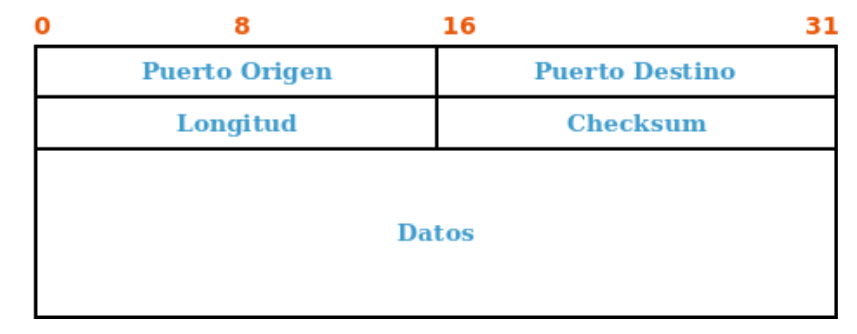
\includegraphics[width=0.7\textwidth]{capitulos/udp/imagenes/datagrama-udp.png}
    \caption{Datagrama de UDP}
    \label{fig:datagrama-udp}
\end{figure}

El tamaño de la \textbf{cabecera} siempre es de \texttt{8 Bytes}, y el checksum es opcional. 

UDP también tiene una \textbf{pseudocabecera} que se añade al principio del datagrama para el cálculo del checksum, pero \textbf{no se envía}. Sirve para comprobar que IP no se haya equivocado en la entrega del datagrama. 

El datagrama de UDP se \textbf{encapsula} en un paquete IP. 



\newpage

\section{Transmission Control Protocol (TCP)}

TCP brinda servicios a las aplicaciones, pero es orientado a conexión. Esto agrega:

\begin{itemize}[label=\textcolor{acento}{$\bullet$}]
    \item Confiabilidad
    \item Ordenado
    \item Control de flujo
    \item Control de congestión
    \item Byte stream
\end{itemize}

Las aplicaciones envían streams de bytes. TCP hace la \textbf{packetization:} convierte el stream en un conjunto de mensajes que IP puede transportar. 

Después decide el tamaño de cada \textbf{chunk} para que no tenga que ser fragmentado. Estos chunks se llaman \textbf{segmentos}. Los segmentos contienen información sobre la posición en el stream, además del proceso origen del nodo emisor y el proceso destino en el nodo destino.

\subsection{Segmento de TCP}

El header del segmento tiene esta forma:

\begin{figure}[htbp]
    \centering
    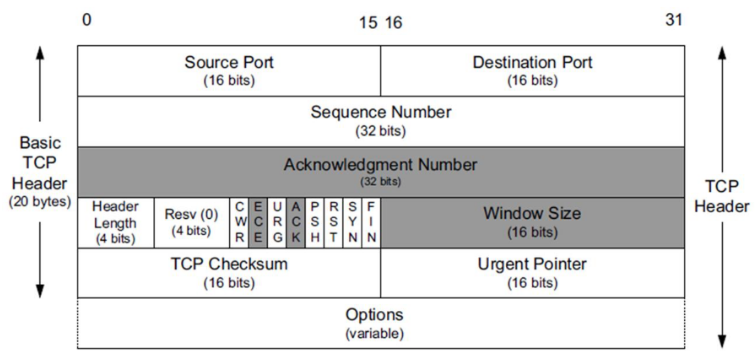
\includegraphics[width=0.7\textwidth]{capitulos/tcp/imagenes/segmento-tcp.png}
    \caption{Segmento TCP}
    \label{fig:segmento-tcp}
\end{figure}

Y sus campos son los siguientes:

\begin{table}[H]
    \centering
    \caption{Campos de la cabecera TCP}
    \label{tab:campos-tcp}
    \renewcommand{\arraystretch}{1.2}
    \begin{tabular}{|p{0.23\textwidth}|p{0.12\textwidth}|p{0.55\textwidth}|}
        \hline
        \textbf{Campo} & \textbf{Tamaño} & \textbf{Descripción} \\ \hline
        Source Port & 16 bits & Indica el número de puerto de la aplicación en el nodo que envía el segmento. \\ \hline
        Destination Port & 16 bits & Indica el número de puerto de la aplicación que debe recibir el segmento. \\ \hline
        Sequence Number & 32 bits & Indica el número asignado al primer byte de datos contenidos en el segmento. \\ \hline
        Acknowledgment Number & 32 bits & Indica el siguiente número de byte que el emisor del segmento espera recibir del otro extremo. \\ \hline
        Header Length & 4 bits & Indica el número de palabras de 4 bytes de la cabecera TCP (entre 20 y 60 bytes). \\ \hline
        Control Bits (Flags) & Variable & También conocidos como \textit{flags}; indican la finalidad del segmento. \\ \hline
        Window Size & 16 bits & Indica la cantidad de bytes, a partir del número de reconocimiento en el segmento, que el emisor puede recibir. \\ \hline
        Checksum & 16 bits & Su cálculo es obligatorio y se realiza sobre todo el segmento más una pseudocabecera. \\ \hline
        Urgent Pointer & 16 bits & Válido si el flag \texttt{U} está seteado. Define el valor a sumar al número de secuencia que indica dónde finalizan los datos urgentes. \\ \hline
        Options & Hasta 40 bytes & Información opcional. \\ \hline
    \end{tabular}
\end{table}

\subsection{Three-Way Handshake}

Se intercambian \textbf{tres segmentos}, donde se indican puertos origen y destino.

\begin{figure}[htbp]
    \centering
    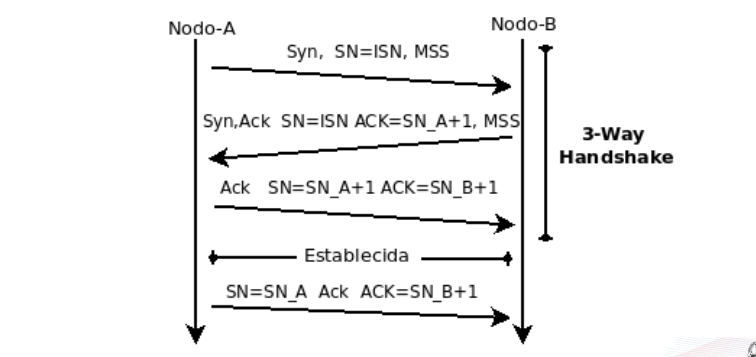
\includegraphics[width=0.7\textwidth]{capitulos/tcp/imagenes/3-way-handshake.png}
    \caption{Three-Way Handshake}
    \label{fig:handshake-tcp}
\end{figure}

\subsubsection{Reset de Conexiones}

Se indica con el \textbf{Flag R} en un segmento, que provoca el cierre inmediato de la conexión. Este reset se puede hacer el cualquier momento, y TCP también lo puede hacer ante determinados eventos. 

El reset es enviado cuando se recibe un segmento que \textbf{no corresponde} a la conexión referenciada. También se envía si se recibe un intento de conexión a un \textbf{puerto cerrado}, a la cual se debe responder con \texttt{Flags R(reset), A (Ack)}.

\subsubsection{Fin de Conexión}

Se intercambian 3 o 4 segmentos para finalizar la conexión, y caulquier extremo puede iniciar el cierre. 

\begin{figure}[htbp]
    \centering
    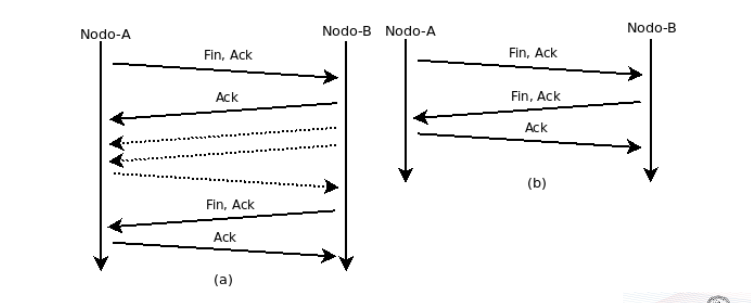
\includegraphics[width=0.7\textwidth]{capitulos/tcp/imagenes/fyn.png}
    \caption{Finalización en TCP}
    \label{fig:fyn-tcp}
\end{figure}

\subsubsection{Estados de TCP}

Durante la conexión, los nodos transitan distintos estados.

\begin{figure}[H]
    \centering
    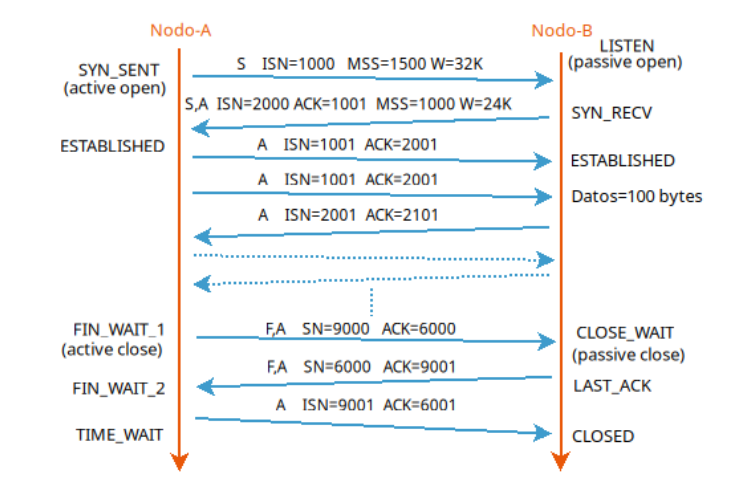
\includegraphics[width=0.7\textwidth]{capitulos/tcp/imagenes/estados-tcp.png}
    \caption{Estados en TCP}
    \label{fig:estados-tcp}
\end{figure}

\begin{nota}{\textbf{\emph{Recordar...}}\newline}
    Las conexiones TCP empiezan con un \textbf{Three-Way Handshake}, con los flags
    
    \begin{enumerate}[label=\textcolor{acento}{\textbf{\arabic*.}}]
        \item SYN
        \item SYN, ACK
        \item ACK
    \end{enumerate}

    El \textbf{Flag de Reset (R)} provoca un cierre instantáneo de una conexión, que se puede volver a abrir. 
    
    Para el \textbf{cierre correcto} de una conexión, también hay un intercambio de 3/4 mensajes.
\end{nota}

\subsection{Intercambio de Datos}

\begin{definicion}{Maximum Segment Size (MSS)}
    Es la máxima longitud de segmento que se puede recibir sin contar la cabecera. Es una opción mandatoria, no es un campo en el header. Se envía en el three-way handshake. 

    Es diferente para \textbf{cada sentido de la conexión}.
\end{definicion}

TCP tiene una \textbf{pseudocabecera} que se construye localmente para el cálculo del checksum. Sirve para verificar la integridad del segmento.

Los \textbf{sequence numbers} son un número de 32 bits cuyo valor de \textbf{ISN} (initial sequence number) se determina localmente en cada extremo. Cada byte enviado sobre una conexión TCP tiene un número de secuencia, y se incrementa según los bytes transmitidos y reconocidos. Indica la ubicación de cada byte en el stream.

\begin{figure}[htbp]
    \centering
    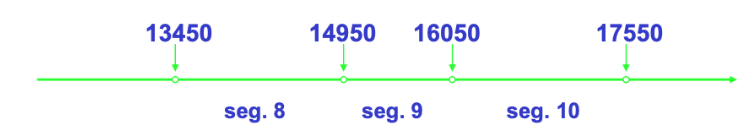
\includegraphics[width=0.7\textwidth]{capitulos/tcp/imagenes/secuencia.png}
    \caption{Secuencias en TCP}
    \label{fig:secuencia-tcp}
\end{figure}

Es un canal \textbf{Full-Duplex} (bidireccional), donde un extremo puede enviar datos hasta que alcance el tamaño de la ventana de recepción sin esperar un ACK. 

El número de ACK indica el siguiente byte que se espera recibir. Si el segmento llega con errores, es retransmitido. 

\begin{nota}{\textbf{\emph{recordar}}\newline}
    Puedo enviar datos hasta llegar a la ventana de transmisión sin tener que esperar un ACK. Si el segmento no tiene errores, me tienen que enviar un ACK. Sino, tengo que retransmitir.
\end{nota}

\subsection{Control de Flujo}

Cada extremo anuncia el tamaño de su \textbf{ventana de recepción} al inicio de la sesión, y pueden ser \textbf{distintos}.

Se utiliza para que un extremo no envíe datos más rápido de lo que el otro extremo los pueda procesar. Si los datos no son leídos por la aplicación, el extremo debe anunciar su ventana de recepción con un menor tamaño.  

\begin{figure}[H]
    \centering
    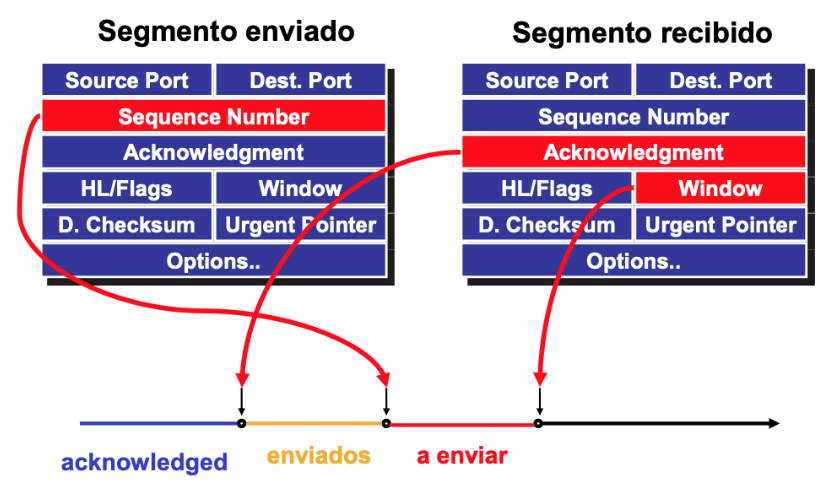
\includegraphics[width=0.7\textwidth]{capitulos/tcp/imagenes/ventana-deslizante.png}
    \caption{Ventana deslizante en TCP}
    \label{fig:ventana-deslizante}
\end{figure}

\begin{definicion}{RTO y RTT}
    \textbf{Round Trip Time:} es el tiempo entre que se envía un segmento y ACK de reconocimiento. El RTT varía continuamente.

    \textbf{Retransmission TimeOut:} el tiempo que debe pasar para retransmitir un paquete. 
\end{definicion}

El \textbf{Maximum Segment Size} se comunica en el campo de \textbf{opciones}, al igual que el escalado de la ventana (\textbf{TCP Windows Scale}). El scale se envía al inicio de sesión, y se va modificando. 

\subsubsection{Timers}

El \textbf{Persist Timer} se utiliza cuando la ventana de recepción se reduce a cero. Una vez que se reduce la ventana, el emisor va enviando paquetes de \textbf{1 Byte} cada un intervalo de tiempo que va incrementando (\textbf{Back-Off}). Esto se hace hasta no recibir un \texttt{ACK} con \texttt{wind = 0}.

El \textbf{Keepalive Timer} sirve para mantener una conexión abierta cuando no hay intercambio de datos. Se utiliza para interrogar al otro extremo por su estado, y funciona de forma muy similar al \emph{persist timer}.

\newpage

\section{QUIC}

QUIC es un protocolo de capa de transporte que viene a solucionar problemas de TCP:

\begin{itemize}[label=\textcolor{acento}{$\bullet$}]
    \item \textbf{Head of Line Blocking:} la pérdida de un segmento bloquea el envío de los segmentos subsiguientes hasta que sea recuperado. 
    \item \textbf{Retardo de Establecimiento de Conexión:} el 3WH tarda mucho. 
    \item \textbf{Tamaño de Cabecera Fijo}. 
    \item \textbf{Identificación de Conexiones:} con TCP se necesita una IP y puerto TCP para identificar una conexión. Si se cambia la IP, el identificador se pierde. 
\end{itemize}

\begin{definicion}{QUIC}
    Protocolo de transporte \textbf{orientado a conexión}, diseñado para permitir intercambios rápidos con \textbf{0-RTT}. Está \textbf{encapsulado en UDP}, pero usa conexiones llamadas \textbf{streams}.
\end{definicion}

\subsection{Paquetes y Frames}

Los extremos se comunican mediante \textbf{paquetes}, y a su vez cada paquete QUIC contiene \textbf{frames}. 

Un datagrama UDP encapsula uno o más paquetes QUIC, un paquete QUIC encapsula uno o más frames de mismo stream o de \textbf{diferentes streams}. 

Hay distintos tipos de paquetes:

\begin{itemize}[label=\textcolor{acento}{$\bullet$}]
    \item \textbf{Version Negotiation:} solo los envía un servidor cuando no conoce la versión de QUIC del cliente.
    \item \textbf{Initial:} transporta el primer frame Crypto entre cliente y servidor, para ejecutar el cambio de claves.
    \item \textbf{0-RTT:} envía datos de aplicación inmediatamente, antes del handshake. Requiere una conexión previa.
    \item \textbf{Retry:} lo envía el servidor cuando queire validar la IP del cliente antes del intercambio de claves.
    \item \textbf{1-RTT:} se usa después de la versión y las claves, contienen streams y acks.
\end{itemize}

\subsection{Streams}

\begin{definicion}{Streams}
    Representa un flujo de bytes dentro de una conexión QUIC, y se crean mediante el envío de datos. Pueden ser creados por cualquiera de los extremos, y la cantidad es arbitraria. Los identifica un Stream ID, que no puede ser reusado durante la conexión. 
\end{definicion}

Los límites de un frame tienen que estar dentro de los límites del \textbf{control de flujo} indicado por el otro extremo. 


\begin{tcolorbox}[
    enhanced,
    colback=blue!3!white,         % Fondo celeste muy suave
    colframe=blue!60!black,       % Borde azul oscuro elegante
    title=\textbf{Ciclo de Vida y Estados de un Stream en QUIC},
    fonttitle=\large\sffamily,    % Fuente del título sin serifas
    coltitle=white,
    boxrule=1.2pt,
    arc=6pt,                      % Bordes redondeados
    drop shadow=black!15!white,   % Sombra sutil
    left=10pt, right=10pt, top=10pt, bottom=10pt
]
En el protocolo QUIC, los \textit{streams} operan como canales lógicos independientes que atraviesan un ciclo de vida estructurado para garantizar la multiplexación eficiente sin sufrir el problema de bloqueo de cabeza de línea (Head-of-Line Blocking). Todo flujo nace en un estado \textbf{Idle} (inactivo) hasta que uno de los extremos inicia la comunicación, pasando al estado \textbf{Open} (abierto), donde ocurre el intercambio de información (unidireccional o bidireccional). A medida que la transmisión de datos finaliza mediante la señalización de un flag \texttt{FIN}, o si la comunicación se interrumpe abruptamente con un \texttt{RESET}, el flujo transita por estados intermedios denominados \textbf{Half-Closed} (semi-cerrado local o remoto), lo que permite que un extremo termine de enviar datos mientras aún sigue recibiendo los del otro lado. Finalmente, cuando ambos sentidos de la comunicación han concluido, el flujo alcanza el estado \textbf{Closed} (cerrado), liberando sus recursos de forma completamente aislada sin afectar la estabilidad ni el rendimiento del resto de los flujos activos en la conexión.

\end{tcolorbox}


\newpage

\section{Domain Name System}

Mapea direcciones (IP/IPv6) a nombres. Los nombres se pueden jerarquizar de dos formas: organizacionalmente y territorialmente. Funciona sobre UDP y utiliza TCP para transferencia de zonas, ambas en puerto 53.

\begin{figure}[H]
    \centering
    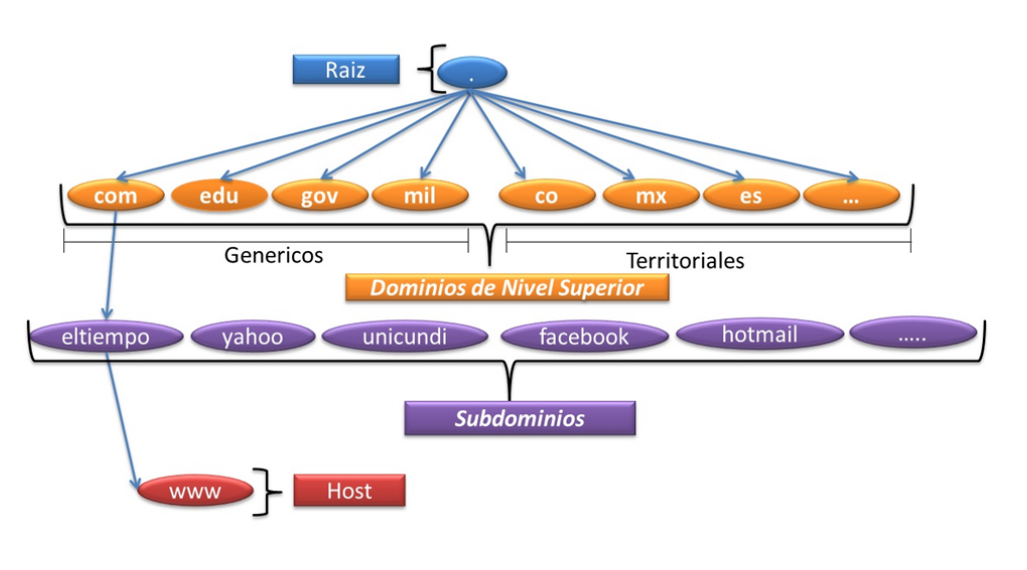
\includegraphics[width=0.5\textwidth]{capitulos/dns/imagenes/jerarquia.png}
    \caption{Jerarquía de nombres DNS}
    \label{fig:dns-jerarquia}
\end{figure}

\begin{definicion}{Zonas}
    Llamamos zona a la undad de administración delegada a un individuo o organización. Es la administración de un determinado espacio de nombres DNS.
\end{definicion}

\begin{figure}[H]
    \centering
    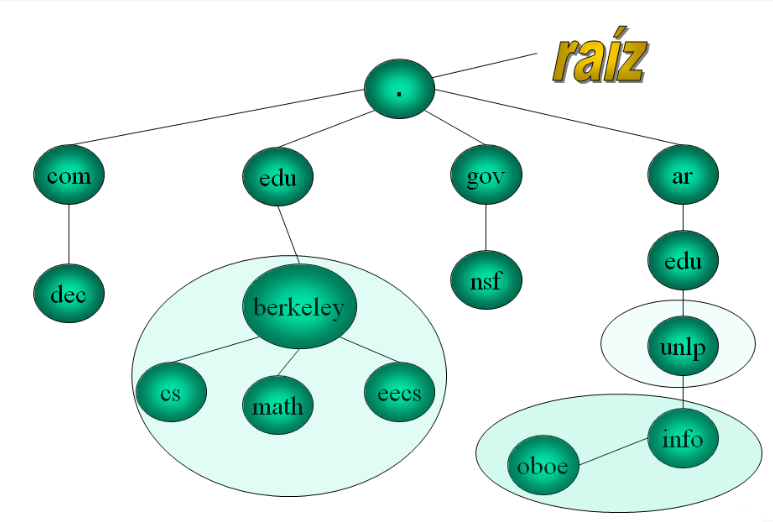
\includegraphics[width=0.5\textwidth]{capitulos/dns/imagenes/zonas.png}
    \caption{Visualización de zonas DNS}
    \label{fig:dns-zonas}
\end{figure}


\subsection{Registros de Recursos}

Son los nombres lógicos con los que se almacenan los datos del servidor.

\begin{itemize}[label=\textcolor{acento}{$\bullet$}]
    \item \textbf{A (Address):} mapea un nombre a una dirección IP.
    \item \textbf{PTR (Pointer):} mapea una dirección IP a un nombre (vice-versa de A).
    \item \textbf{CNAME (Canonical Name):} apunta a otro nombre, se lo conoce como \emph{alias}.
    \item \textbf{MX (Mail Exchanger):} registro que hace funcionar al correo electrónico. Le dice a todo Internet \textbf{qué servidor es el encargado de recibir los mails} de ese dominio.
    \item \textbf{NS (Name Server):} indica cuáles son los servidores DNS que tienen la información oficial y actualizada.
    \item \textbf{SOA (Start Of Authority):} para pedir parámetros del dominio.
\end{itemize}

\subsection{Servidores DNS}

El \textbf{servidor raíz} delega a todos TLDs, y no permite consultas recursivas. Proporcionan referencias directas a servidores dedominio de segundo nivel (com, edu, gov, ...). Los \textbf{servidores autoritativos} se encargan de una zona o sub-dominio de nombres, y puede subdelegar.

Los \textbf{servidores locales} son los que se consultan dentro de una red. Mantienen caché, permiten consultas recursivas a los hosts internos y pueden ser autoritativos. 

Luego están los \textbf{Open Name Servers}, que son servidores de DNS que funcioan como si fueran locales para cualquier cliente. Los \textbf{Forwarded Name Servers} funcionan como proxies de otros DNSs internos, e interactúan directamente con el sistema DNS exterior.

Los \textbf{Primary Name Servers} almacenan la información de su zona en una database local, y son responsables de mantener la información actualizada. Los \textbf{Secondary Name Servers} obtienen los datos desde otro servidor que tenga la autoridad para esa zona, y copia la información. Este proceso se llama \emph{transferencia de zona} y en vez de hacerse por UDP se hace por TCP.

\subsection{Proceso de Consulta}

\begin{tcolorbox}[
    enhanced,
    colback=green!2!white,        % Fondo verde muy suave
    colframe=green!50!black,      % Borde verde oscuro elegante
    title=\textbf{Mecanismo de Resolución de Nombres (DNS)},
    fonttitle=\large\sffamily,    % Fuente del título sin serifas
    coltitle=white,
    boxrule=1.2pt,
    arc=6pt,                      % Bordes redondeados
    drop shadow=black!15!white,   % Sombra sutil
    left=10pt, right=10pt, top=10pt, bottom=10pt
]

Todo host cuenta con la configuración de un \textbf{servidor DNS local} (resolver). Cuando un dispositivo necesita resolver un nombre de dominio, envía su petición inicial a este servidor local, a partir de lo cual pueden darse dos escenarios:

\begin{itemize}[leftmargin=*, label=\textcolor{green!50!black}{\textbullet}]
    \item \textbf{Respuesta Autoritativa (Fidedigna):} Si el servidor local es la autoridad para el dominio consultado, significa que aloja exactamente esa porción de la base de datos distribuida. En este caso, posee el mapeo directo y le devuelve la respuesta al host de forma inmediata.
    
    \item \textbf{Búsqueda Externa (Delegación):} Si el servidor local no es fidedigno para dicho dominio, deberá iniciar una búsqueda externa consultando a un \textbf{Root Server} (Servidor Raíz).
\end{itemize}

\vspace{0.2cm}
\noindent\textbf{Dinámica de Peticiones (Recursivas vs. Iterativas):} \\
Para evitar la sobrecarga y el colapso de la infraestructura global, la petición dirigida al Root Server es estrictamente \textbf{iterativa}. El Root Server no busca la IP final, sino que se limita a devolver la dirección de un servidor intermedio (como un servidor TLD). 

A partir de allí, el servidor local envía una petición \textbf{recursiva} a este servidor intermedio. Al ser recursiva, le delega la responsabilidad de continuar interrogando a la jerarquía de servidores hasta alcanzar al servidor fidedigno definitivo. Una vez hallado el mapeo correcto, la respuesta viaja de regreso hasta llegar al host original.

\end{tcolorbox}

Se utiliza \textbf{Caching} para reducir el tráfico en búsquedas de dominios no locales, donde las entradas a esta memoria se temporizan.  

\subsection{Flags DNS}

Cuando realizamos una \textbf{consulta DNS}, la misma puede retornar distintos flags.

\begin{itemize}[leftmargin=*, label=\textcolor{acento}{$\bullet$}]
    \item \textbf{qr:} query.
    \item \textbf{rd:} recursion desired, el cliente desea que la consulta se resuelva recursivamente.
    \item \textbf{ra:} recursion available, el servidor tiene la recursión habilitada.
\end{itemize}

El \textbf{TTL} (Time to Live) indica el tiempo que se mantiene la respuesta en caché (en segundos).



\newpage

\section{File Transfer Protocol - FTP}

\begin{definicion}{FTP}
    Protocolo utilizado para \textbf{compartir y acceder a archivos}. Se encapsula en TCP en puerto 20 y 21 para las conexiones de control y transferencia. 
\end{definicion}

El cliente utiliza un puerto TCP aleatorio, mientras que el servidor utiliza el \textbf{21 para el control} y el \textbf{20 para transferencia}. 

\newpage

\section{Correo Electrónico}

Hay tres protocolos principales para el correo electrónico, con distintos fines:

\begin{itemize}[label=\textcolor{acento}{$\bullet$}]
    \item \textbf{Distribución:} se utiliza el protocolo SMTP o Extended SMTP (ESMTP).
    \item \textbf{Entrega Final:} permite al usuario gestionar su correo a través de una máquina remota. Son POP3, IMAP o HTTP.
\end{itemize}

\begin{figure}[htbp]
    \centering
    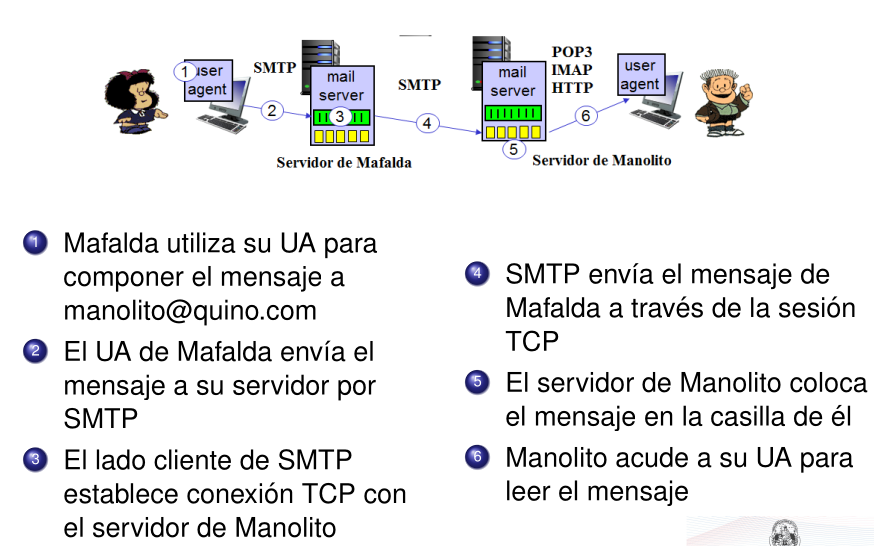
\includegraphics[width=0.8\textwidth]{capitulos/correo/imagenes/ciclo.png}
    \caption{Ciclo de un Correo Electrónico}
    \label{fig:ciclo-correo}
\end{figure}

\subsection{Simple Mail Transfer Protocol - SMTP}

\begin{definicion}{Definición}
    Tiene el objetivo de transferir mails de manera confiable y segura. El usuario coloca una copia del mensaje en el \emph{spool} y el cliente en \emph{background} envía los mensajes. El cliente barre los mensajes cada un cierto tiempo.  
\end{definicion}

Se utiliza DNS para resolver el nombre del destino en una dirección IP y luego se establece la conexión TCP con el servidor. 

\begin{enumerate}[label=\textcolor{acento}{\textbf{\arabic*.}}]
    \item El sender abre una conexión TCP al \textbf{puerto 25 del receptor}. 
    \item El \textbf{User Agent} consulta por el registro A de su servidor DNS.
    \item El \textbf{SMTP Server} hace una consulta DNS para obtener los registros \textbf{MX} del dominio destino. 
    \item Hacen un handshake entre el receptor y el emisor. 
\end{enumerate}

\subsubsection{Multipurpose Internet Mail Extensions - MIME}

\begin{definicion}{MIME}
    Es una extensión para enviar archivos ejecutables y multimedia mediante mail con ASCII de 7 bits, que era lo que permitía SMTP.
\end{definicion}


\subsection{Post Office Protocol 3 - POP3}

\begin{definicion}{POP3}
    Tiene como objetivo obtener el correo electrónico del buzón remoto y almacenarlo localmente en la PC del usuario para su lectura. Utiliza el \textbf{TCP en puerto 110}. 
\end{definicion}

Puede ser \emph{download and delete} o \emph{download and keep}. Según la modalidad borra o no los mensajes en la fase de actualización. En caso de que esté en \emph{download and delete}, no permite sincronismo entre otros dispositivos. 

\subsection{IMAP}

\begin{definicion}{IMAP}
    Asocia cada mensaje a una carpeta, sobre las cuales se pueden desplazar los mails. A diferencia de POP3, permite sincronismo entre otros dispositivos, ya que se accede al servidor para leer y no se borran los leídos.
    
    Funciona sobre \textbf{TCP en puerto 143}.
\end{definicion}

También incorpora descargas parciales de los mensajes. 

\newpage

\section{Hypertex Transfer Protocol - HTTP/1.1}

Es el protocolo encargado de transferir \textbf{recursos} en internet. Los recursos son identificados por una \textbf{URI} (Uniform Resource Location). Las URIs tienen dos formatos: URN (Uniform Resource Name) o URL (Uniform Resource Location).

\begin{tcolorbox}[
    enhanced,
    colback=blue!3!white,         % Fondo celeste muy suave
    colframe=blue!60!black,       % Borde azul oscuro elegante
    title=\textbf{Funcionamiento de HTTP},
    fonttitle=\large\sffamily,    % Fuente del título sin serifas
    coltitle=white,
    boxrule=1.2pt,
    arc=6pt,                      % Bordes redondeados
    drop shadow=black!15!white,   % Sombra sutil
    left=10pt, right=10pt, top=10pt, bottom=10pt
]
Es un protocolo de solicitud/respuesta \textbf{sin estado}, de \textbf{texto plano}. Utiliza MIME para enviar datos binarios. Corre sobre \textbf{TCP puerto 80}. También existe una versión segura \textbf{HTTPS} que usa TLS; corre en \textbf{TCP puerto 443}. 

Cuando se solicita un recurso tenemos que esperar la respuesta, no hay un identificador que permita relacionarlas. Permite \emph{pipelining}.
\end{tcolorbox}

\subsection{Mensajes y Métodos}

\begin{enumerate}[label=\textcolor{acento}{\textbf{\arabic*.}}]
    \item Los clientes envían \textbf{request methods} al servidor mediante HTTP. Este request method indica al servidor qué acción ejecutar.
    \item El servidor ejecuta el method.
    \item El servidor responde con uno o más \textbf{response methods} que incluyen un código de estado, indicando si la solicitud fué exitosa o no, o si debe realizar alguna acción.
\end{enumerate}

Los mensajes tienen la misma estructura: línea de inicio, cabecera y cuerpo (opcional). 

\begin{figure}[H]
    \centering
    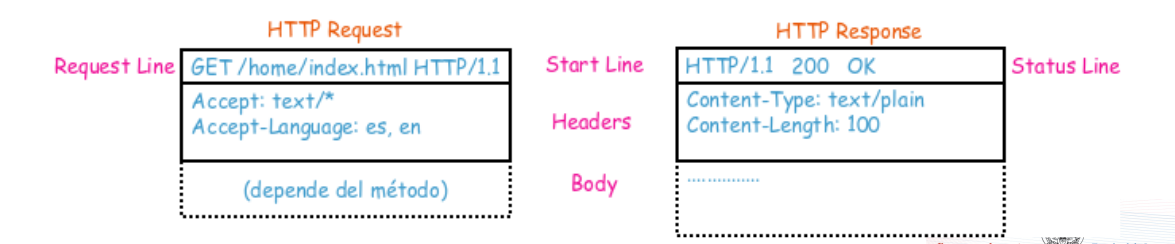
\includegraphics[width=0.8\textwidth]{capitulos/http1/imagenes/mensaje.png}
    \caption{Mensajes HTTP/1.1}
    \label{fig:http-mensaje}
\end{figure}

La \textbf{línea de inicio} es la primera de todos los mensajes HTTP, luego siguen las \textbf{cabeceras} de nombre-valor separadas por \texttt{:}, y por último el \textbf{body} que depende del método usado y del resultado de la operación. 

\subsubsection{Algunos Métodos}

Los métodos más utilizados son:

\begin{itemize}[label=\textcolor{acento}{$\bullet$}]
    \item \textbf{GET:} el cliente solicita un recurso al servidor. Podrían enviarse datos en el body, pero no es usual. Ejemplo: \texttt{http://www.example.com/index.php?pais=Argentina,deporte=tenis}. Los parámetros van después del \texttt{?}.
    \item \textbf{HEAD:} igual al GET pero solo se obtienen los \textbf{metadatos} del recurso (headers). No se envía el recurso solicitado.  
    \item \textbf{POST:} envía datos de entrada al servidor, que se mandan en el body. Solicita una respuesta del servidor.
    \item \textbf{PUT:} envía contenido que será almacenado en el webserver. 
    \item \textbf{DELETE:} indica contenido a ser eliminado del webserver.  
\end{itemize}

\subsection{Funcionamiento}

Cada mensaje puede tener ninguna o muchas cabeceras que agregan información adicional a los mensajes. Algunas cabeceras son:

\begin{itemize}[label=\textcolor{acento!60}{$\bullet$}]
    \item \textbf{Host:} obligatoria, infica el servidor y puerto destino.
    \item \textbf{Date:} día y hora de creación del mensaje.
    \item \textbf{Content-Lenght:} longitud del cuerpo del mensaje.
    \item \textbf{Content-Type:} tipo de objeto que se envía.
\end{itemize}

\begin{figure}[H]
    \centering
    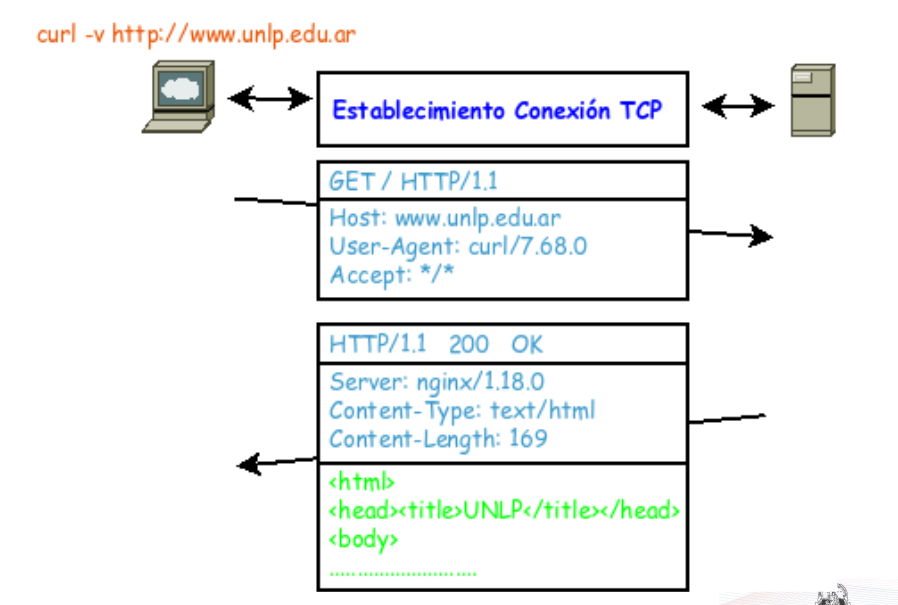
\includegraphics[width=0.8\textwidth]{capitulos/http1/imagenes/funcionamiento.png}
    \caption{Funcionamiento de HTTP/1.1}
    \label{fig:http-funcionamiento}
\end{figure}

\begin{nota}{\emph{\textbf{Recordar...}}\smallskip}
    En \textbf{HTTP/1.0} las conexiones eran \textbf{no persistentes}, es decir, se transfiere un objeto por cada sesión y por cada recurso se debe abrir y cerrar una sesión TCP. El servidor responde con un objeto y cierra la sesión (algunas implementaciones de HTTP/1.0 soportan conexiones keep-alive, pero no es lo default).
\end{nota}

En HTTP/1.1 las conexiones son \textbf{persistentes por defecto}, y con las cabeceras \emph{Connection: close} indicamos que queremos cerrar la conexión después de la respuesta del server. 

\begin{figure}[H]
    \centering
    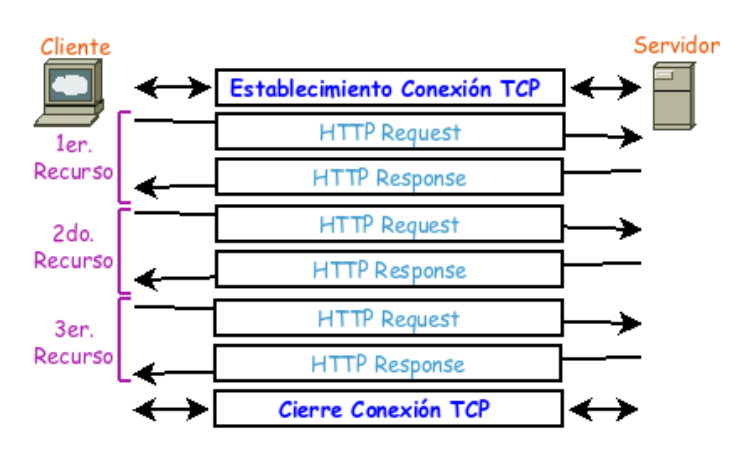
\includegraphics[width=0.8\textwidth]{capitulos/http1/imagenes/conexiones-persistentes.png}
    \caption{Conexiones persistentes de HTTP/1.1}
    \label{fig:http-conexiones-persistentes}
\end{figure}

\begin{definicion}{Concurrencia en HTTP/1.1}
    Este protocolo permite \textbf{pipelining:} el cliente puede enviar muchas solicitudes sin esperar cada respuesta, y el servidor las procesa en paralelo. Tiene que enviar las respuestas en el \textbf{mismo orden} que recibió las solicitudes.
    
    Los clientes pueden abrir \textbf{conexiones simultáneas} a un servidor, usadas para evitar el \emph{head-of-line blocking}.    
\end{definicion}

Se puede hacer un \textbf{GET Condicional} con la cabecera \texttt{If\_Modified\_Since}, donde el servidor retorna el recurso si fué modificado en una fecha posterior a la indicada en el header. Si no fue modificada, se responde con código \texttt{304} y el recurso se recupera de caché.

Si el recurso fué designado a una nueva URL, el server responde con \texttt{301 (Moved Permanently)} o \texttt{302 (Found)}, y agrega una cabecera \texttt{Location} con la nueva URL.

\subsection{HTTPS}

Es HTTP con TLS, sobre TCP en puerto 443. Los mensajes HTTP se \textbf{encriptan y autentican de forma completa}. 

\begin{figure}[H]
    \centering
    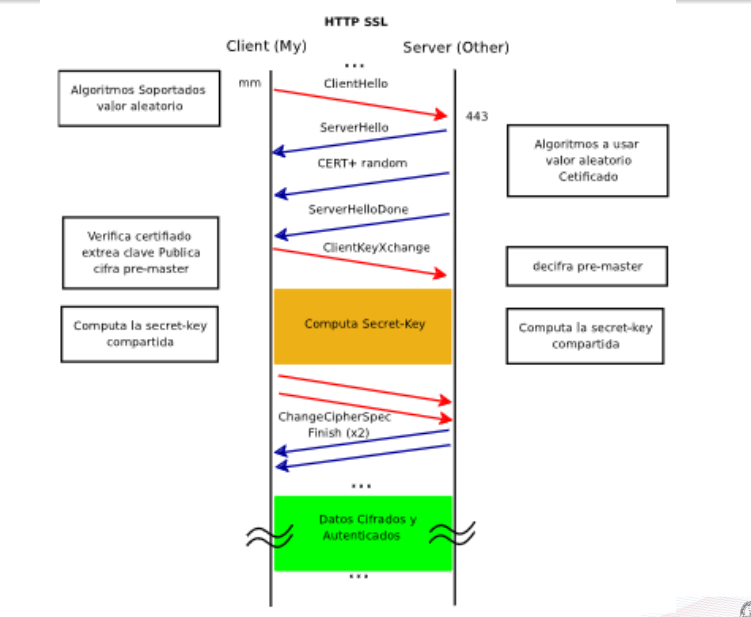
\includegraphics[width=0.8\textwidth]{capitulos/http1/imagenes/https.png}
    \caption{TLS en HTTP/1.1 (HTTPS)}
    \label{fig:http-https}
\end{figure}

\subsection{Cookies}

Las cookies permiten a las aplicaciones web del server \textbf{manejar estados} conservando información entre peticiones del cliente, ya que HTTP/1.1 no maneja estados por defecto. 

Los servers envían información de estado con un header \texttt{Set-Cookie}, y en las siguientes solicitudes el cliente retorna una cabecera \texttt{Cookie} con los datos recibidos.

\begin{figure}[H]
    \centering
    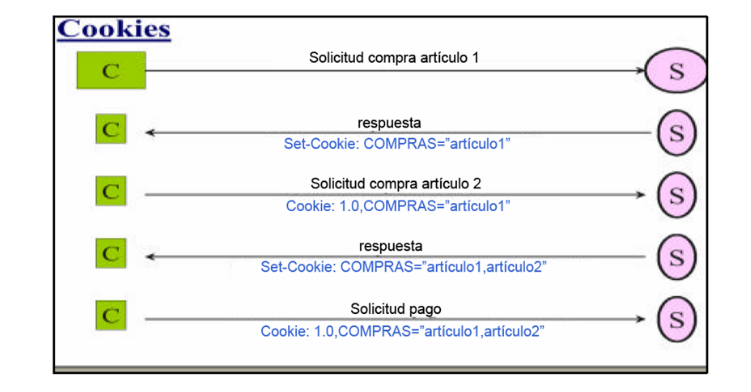
\includegraphics[width=0.6\textwidth]{capitulos/http1/imagenes/cookies.png}
    \caption{Ejemplo de uso de Cookies}
    \label{fig:http-cookies}
\end{figure}

\subsection{Caching}

Es una característica opcional de HTTP/1.1 que consiste en almacenar de forma local los mensajes de respuesta para reducir el tiempo de respuesta y carga de la red. 

Hay que asegurar que los contenidos guardados en caché sean equivalentes a los almacenados en el servidor, generalmente almacenan respuestas exitosas de una solicitud de recuperación. 

Si la solicitud es servida desde cache se conoce como \textbf{cache hit}, y si no se encuentra en la cache es un \textbf{cache miss} y se pide el recurso al webserver. Cuando el recurso está en la caché pero no es válido, se tiene que revalidar utilizando un \texttt{GET} condicional. 

\newpage

\end{document}